\let\negmedspace\undefined
\let\negthickspace\undefined
\documentclass[journal]{IEEEtran}
\usepackage[a5paper, margin=10mm, onecolumn]{geometry}
%\usepackage{lmodern} % Ensure lmodern is loaded for pdflatex
\usepackage{tfrupee} % Include tfrupee package

\setlength{\headheight}{1cm} % Set the height of the header box
\setlength{\headsep}{0mm}     % Set the distance between the header box and the top of the text

\usepackage{gvv-book}
\usepackage{gvv}
\usepackage{cite}
\usepackage{amsmath,amssymb,amsfonts,amsthm}
\usepackage{algorithmic}
\usepackage{graphicx}
\usepackage{textcomp}
\usepackage{xcolor}
%\usepackage{txfonts}
\usepackage{listings}
\usepackage{enumitem}
\usepackage{mathtools}
\usepackage{gensymb}
\usepackage{comment}
\usepackage[breaklinks=true]{hyperref}
\usepackage{tkz-euclide} 
\usepackage{listings}
% \usepackage{gvv}                                        
\def\inputGnumericTable{}                                 
\usepackage[latin1]{inputenc}                                
\usepackage{color}                                            
\usepackage{array}                                            
\usepackage{longtable}                                       
\usepackage{calc}                                             
\usepackage{multirow}                                         
\usepackage{hhline}                                           
\usepackage{ifthen}                                           
\usepackage{lscape}
\usepackage{circuitikz}
\tikzstyle{block} = [rectangle, draw, fill=blue!20, 
    text width=4em, text centered, rounded corners, minimum height=3em]
\tikzstyle{sum} = [draw, fill=blue!10, circle, minimum size=1cm, node distance=1.5cm]
\tikzstyle{input} = [coordinate]
\tikzstyle{output} = [coordinate]


\begin{document}

\bibliographystyle{IEEEtran}
\vspace{3cm}

\title{4.12.44}
\author{AI25BTECH11030 -Sarvesh Tamgade}
{\let\newpage\relax\maketitle}

\renewcommand{\thefigure}{\theenumi}
\renewcommand{\thetable}{\theenumi}
\setlength{\intextsep}{10pt} 


\numberwithin{equation}{enumi}
\numberwithin{figure}{enumi}
\renewcommand{\thetable}{\theenumi}


\textbf{Question}: Find the equation of the set of points which are equidistant from the points \(\vec{A} = \myvec{1 \\ 2 \\ 3}\) and \(\vec{B} = \myvec{3 \\ 2 \\ -1}\).


\textbf{Solution:} \
Let \(\vec{X}\) be the position vector of any point equidistant from \(\vec{A}\) and \(\vec{B}\).
The equidistance condition is
\begin{align}
\|\vec{X} - \vec{A}\| = \|\vec{X} - \vec{B}\|.
\end{align}
Squaring both sides, we have
\begin{align}
(\vec{X} - \vec{A})^\top (\vec{X} - \vec{A}) = (\vec{X} - \vec{B})^\top (\vec{X} - \vec{B}).
\end{align}
Expanding and simplifying,
\begin{align}
\vec{X}^\top \vec{X} - 2 \vec{A}^\top \vec{X} + \vec{A}^\top \vec{A} = \vec{X}^\top \vec{X} - 2 \vec{B}^\top \vec{X} + \vec{B}^\top \vec{B},
\end{align}
which reduces to
\begin{align}
-2 \vec{A}^\top \vec{X} + \vec{A}^\top \vec{A} = -2 \vec{B}^\top \vec{X} + \vec{B}^\top \vec{B}.
\end{align}
Rearranging,
\begin{align}
2 (\vec{B} - \vec{A})^\top \vec{X} = \vec{B}^\top \vec{B} - \vec{A}^\top \vec{A}.
\end{align}
Calculate the vector difference:
\begin{align}
\vec{B} - \vec{A} = \myvec{3 - 1 \\ 2 - 2 \\ -1 - 3} = \myvec{2 \\ 0 \\ -4} = 2 \myvec{1 \\ 0 \\ -2}.
\end{align}
Calculate the scalar values:
\begin{align}
\vec{B}^\top \vec{B} = 3^2 + 2^2 + (-1)^2 = 14, \quad \vec{A}^\top \vec{A} = 1^2 + 2^2 + 3^2 = 14,
\end{align}
so the right side is zero:
\begin{align}
\vec{B}^\top \vec{B} - \vec{A}^\top \vec{A} = 0.
\end{align}
Thus, substituting the simplified difference vector, the plane equation becomes:
\begin{align}
4\myvec{1 & 0 & -2}\vec{X} = 0,
\end{align}
or equivalently,
\begin{align}
\myvec{1 & 0 & -2}\vec{X} = 0.
\end{align}
\textbf{Final Answer:} The set of points equidistant from \(\vec{A}\) and \(\vec{B}\) lies on the plane defined by
\[
\boxed{
\myvec{1 & 0 & -2} \vec{x} = 0
}
\]


\begin{figure}[htbp]
    \centering
    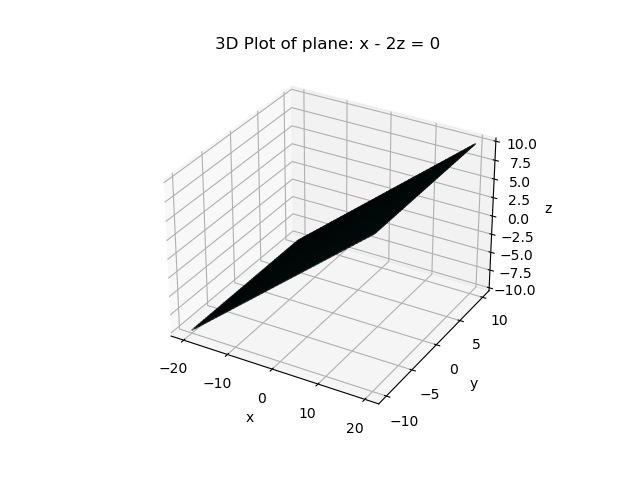
\includegraphics[width=0.65\linewidth]{FIG/fig1.png}
    \caption{Vector Representation}
    \label{fig:FIG/fig1.png}
    \end{figure}

\end{document}  